\documentclass[10pt,a4paper,twoside]{article}
\usepackage[a4paper,top=20mm,bottom=20mm,outer=5cm]{geometry}
\usepackage[utf8]{inputenc}
\usepackage[english]{babel}
\usepackage{graphicx}
\usepackage{hyperref}
\usepackage{amsmath}
\usepackage{acronym}
\usepackage{cleveref}
\usepackage{natbib}
\bibliographystyle{abbrvnat}
\setcitestyle{authoryear}


\title{Project Machine Learning\\--- Milestone 1 ---}

%%%%%%%%%%%%%%%%%%%%%%%%%%%%%%%%%%%%%%%
%                                     %
%   EVERYTHING BELOW CAN BE CHANGED   %
%                                     %
%%%%%%%%%%%%%%%%%%%%%%%%%%%%%%%%%%%%%%%

\author{Konstantin Ausborn, Timon Palm, Marco Rosinus Serrano}
\date{\today}

\acrodef{ae}[AE]{Autoencoder}
    \acrodef{vae}[VAE]{Variational Autoencoder}
    \acrodef{vq}[VQ-VAE]{Vector Quantized Variatonal Autoencoder}
    \acrodef{gan}[GAN]{Generative Adversarial Networks}
    \acrodef{dnn}[DNN]{Deep Neural Networks}
    \acrodef{bpp}{bits per pixel}
    \acrodef{mse}[MSE]{Mean Squared Error}
    \acrodef{psnr}[PSNR]{Peak Signal to Noise Ratio}
    \acrodef{nll}[NLL]{Negative Log Likelihood}

\begin{document}

    \maketitle

    \section{Baseline method and evaluation}\label{sec:baseline-method-and-evaluation}
    The \ac{vq} described in the paper both learns useful and compact, discrete representations of real world data,
and generates new samples in this representation space and decoding them back to the original data space.
The paper mainly focuses on the generative aspect, but to understand the whole model better, we want to gain insights
into both, and chose our baseline methods accordingly.

\subsection{Baselines}\label{subsec:baselines}
While there exist multiple machine learning approaches with a setup similar to that of the \ac{vq}
i.e.\ generative models with latent representations such as \ac{gan}, differences in the details make these hard to
compare against each other.
When sticking to the example of \ac{gan}, one key difference is that in the basic model, the latents can not be created
by encoding real world data but overall represent a distribution that is close to that of the training data~\cite{gan}.

Another requirement for or baseline model is some simplicity.
Since it is the original model that the non-quantized \ac{vae} is based on, which in turn later was developed into the
\ac{vq} and because it also fulfils the requirement of simplicity, we chose the basic \ac{ae} as our general baseline
method.
We also incorporate some experiments with the \ac{vae}, to show the progress that was made over time.

The similar architecture of these baselines allow for very comparable results, since they can be tuned to be very
close in size, training cost and latent structure.
When constructing the neural network, we adhered to the same architecture as the \ac{vq} wherever possible,
only deviating where it is absolutely necessary, directly around the latent layer.


While much of the current work in realistic high resolution image generation is based on \ac{dnn} \cite{citationNeeded},
the field of image compression is well researched both in-, and outside deep architectures~\cite{compression},
and non-ML approaches are still dominant on the web as can be seen in Figure~\ref{fig:file_formats}.
To represent this, we also use the popular JPEG format for comparisons against our lossy compression schemes.

\begin{figure}[H]
    \centering
    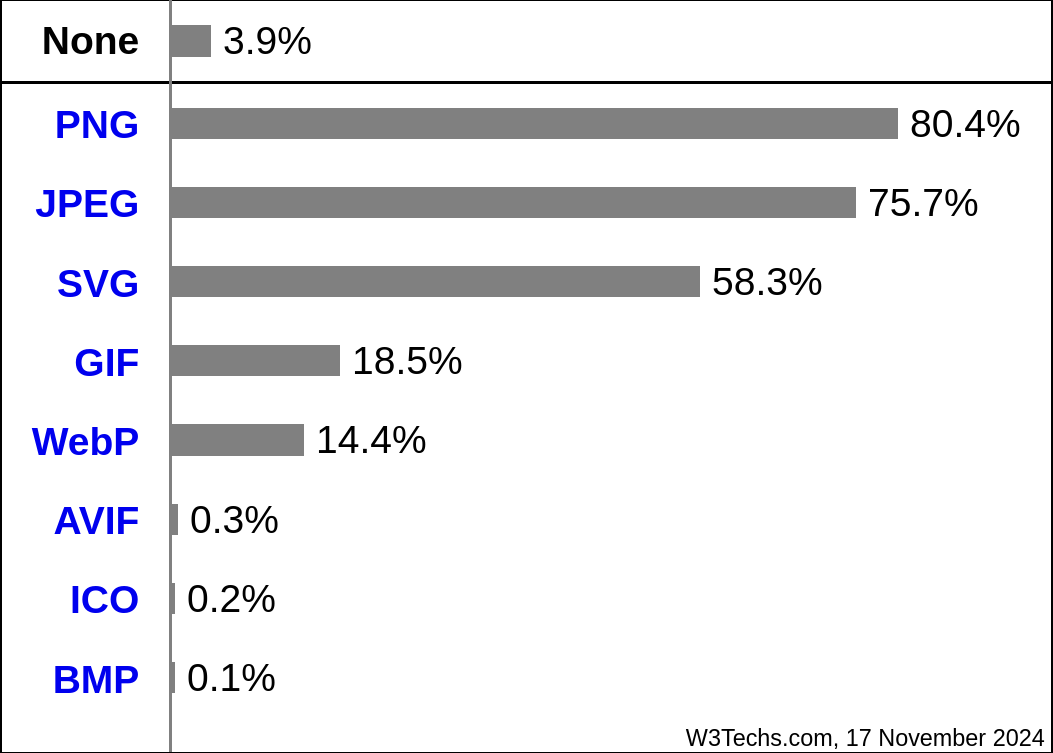
\includegraphics[width=0.5\textwidth]{images/formats}
    \caption{Percentages of websites using various image file formats~\cite{img_file_format}}
    \label{fig:file_formats}
\end{figure}

\subsection{Evaluation Metrics}\label{subsec:evaluation-metrics}

\subsubsection{Compression}
For compression, the most straightforward metric is to measure the reduction of memory required to
store the data.
To normalize over image resolution, we choose to evaluate the \ac{bpp}.

The second, and less objective measure, is image similarity after reconstruction.
While the \ac{mse} and by transfer \ac{psnr} describe pixel-wise similarity very well, it is not
always optimal to judge perceived similarity for humans, as can be seen in Figure~\ref{fig:mse_ssim}.

\begin{figure}[ht]
    \centering
    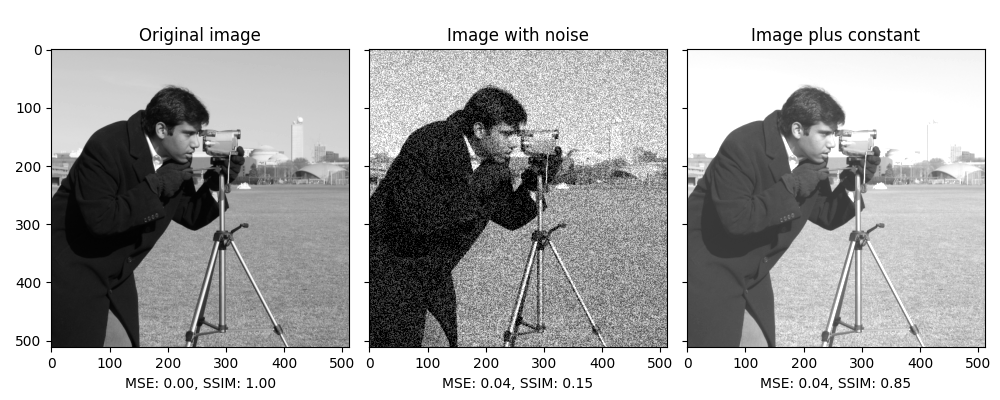
\includegraphics[width=0.8\textwidth]{images/ssim_mse}
    \caption{from~\cite{scikit-ssim}}
    \label{fig:mse_ssim}
\end{figure}

To overcome these limitations we will use the \ac{ssim}, a metric working under the assumption that human visual
perception is highly adapted for extracting structural information from a scene, that has been

Even though this analysis favours \ac{ssim}, we use \ac{mse} as our loss function for our baseline models,
since the \ac{vq} implementation we plan to replicate does the same, and we want to maximize comparability.
We use \ac{ssim} for result evaluation, and add \ac{psnr} values for further work later on.

\subsubsection{Image Generation}
An important metric in Image Generation and the one used to argue about the strong performance of the \ac{vq} in the
paper is the \ac{nll} normalized to the amount of pixels (dimensions) in an image, given in bits/dim.
A lower number indicates a higher likelihood of generating the test data given our model.
The bits/dim number is rooted in information theory, and describes the average number of bits required to
compress the test data with the entropy coding scheme that is optimal for a model~\cite{shannon}.

The \ac{fid}, introduced by~\cite{fid}, is another interesting metric.
It compares the distribution of features of a generator with that of real images via a network trained on a big
dataset, often also imagenet.

Another criterion not to be left out is the classic human turing test, as in evaluating the images by hand.
Even though this is not scalable, it is the ultimate classifier for human perception, and can be a good starting
point.

As on metrics we found, but decided not to use: The paper that introduced \ac{fid} it also shows that it is more
consistent than a previous, similar metric, the inception score, which we will therefore leave out.
Another sometimes utilized evaluation metric that research has shown to better avoid are Parzen Windows Estimates~
\cite{note_on_eval}.

Overall, since we have not yet implemented any Image Generation functionality, it remains to be seen which of these
criteria are of which worth to us.

MY QUESTIONS: MORE FORMULAE FOR THE CRITERIONS?

\subsection{VAE}
Our version of the VAE follows the same basic structure as the Autoencoder
previously described. First we use 2 convolutional layers to downsample the
image to $1/4$ of its original height and width. Then two convolutional
residual blocks are applied, each of which contains two convolutional layers.
An important difference of the VAE is that its encoder outputs a random
variable $\boldsymbol{\hat{z}} \sim \mathcal{N}(\boldsymbol{\mu_\theta}, \text{diag}
(\boldsymbol{\sigma_\theta}))$. $\boldsymbol{\hat{z}}$ is obtained using the
reparameterization trick, which consists in sampling $\boldsymbol{z}
\sim \mathcal{N}(0, I)$ and then computing $\boldsymbol{\hat{z}} =
\boldsymbol{\mu_\theta} + \boldsymbol{z} \odot \boldsymbol{\sigma_\theta}$.
$\boldsymbol{\mu_\theta}$ and $\boldsymbol{\sigma_\theta}$ are deterministic
outputs of the last convolutional layer of the VAE's encoder. This allows to
optimize the model using the ELBO loss which in turn enables us to not only
reconstruct the input, but to learn a posterior distribution $p(x|z)$ while
the encoder $q(z|x)$ tries to be as close as possible to $p(z)$. Thus enabling
us to generate new dataset samples by sampling $z \sim p(z)$ and then feeding
it through the decoder.

\subsection{Overfitting}\label{subsec:overfitting}
Overfitting in the context of machine learning refers to the phenomenon where
a model instead of learning useful features from the training data, that
generalize to unseen data, it starts "memorizing" the training data. This
leads to bad performance on the test set. While theoretically, this may still
be an issue with autoencoders and VAEs, we have not experienced this happening
when training with normal settings. This is very likely due to the large
dataset size and the inductive bias of the convolution operation.

\subsection{Class differences}

\subsection{What constitutes good features in machine learning}
In classical machine learning, a set of features is "good", if it helps the
model to achieve a certain task. This implies that the features should be
informative, meaning that they should have some predictive value towards our
final goal. In simple regression settings, this is the case if the feature
correlates with the true value. Furthermore it is helpful for features to be
independent form each other. Dependent features could overemphasize their
importance due to the higher frequency. And lastly, features should be simple.
A classical example would be the task of delivery time prediction between two
locations. Here it is advised to use the distance between the two locations
instead of passing a pair of coordinates, which would cause the model to first
extract knowledge about the distance of the locations. Another important thing
to think of is normalization. Features that intrinsically live on a scale
magnitudes larger than other features will have higher impact on the final
output and will therefore be considered "more important" than other features.

The above listed reasons all are due to the fact that traditional ML models
usually are very sensitive to small perturbations which calls for efficient
feature engineering. In modern deep learning settings this is not so much the
case. Here we see that the models generally become insensitive to small
perturbations in the data. Thats why there is generally not much preprocessing
done. Most commonly the data is normalized into a [-1, 1] range.


    \section{Discussion}
    :-)
    \bibliography{bibliography}
\end{document}
